\documentclass{standalone}
\usepackage[utf8]{inputenc}
\usepackage{amsmath}
\usetikzlibrary{calc,positioning}

\begin{document}

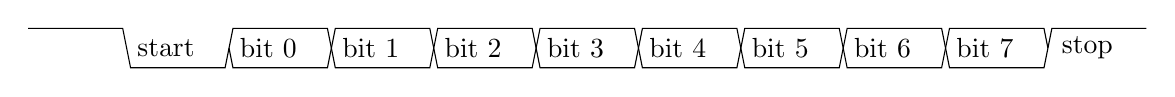
\begin{tikzpicture}
		\coordinate(x) at (0,0);
		\draw
			(x) -- ++(1.2,0) -- ++(0.05,-0.25) coordinate (x);
		\draw
			($(x)+(0.5,0)$) node {start}
			(x)-- ++(0.05,-0.25) -- ++(1.2,0) -- ++(0.05,0.25) coordinate (x);
		\foreach \x in {0,1,2,3,4,5,6,7}{
			\draw ($(x)+(0.5,0)$) node {bit \x}
				(x)-- ++(0.05,0.25) -- ++(1.2,0) -- ++(0.05,-0.25)
				(x)-- ++(0.05,-0.25) -- ++(1.2,0) -- ++(0.05,0.25)
				coordinate (x);
			}
		\draw
			($(x)+(0.5,0)$) node {stop}
			(x)-- ++(0.05,0.25) -- ++(1.2,0) coordinate (x);
\end{tikzpicture}

\end{document}
